\documentclass{bioinfo}
\copyrightyear{2014}
\pubyear{2014}
\usepackage{url}

\begin{document}
\firstpage{1}

\title[ADAM: Cloud Scale Genomic Processing]{ADAM: A Data Format And Pipeline For Cloud Scale Genomic Processing}
\author[Massie \textit{et~al}]{Matt~Massie\,$^{1,*}$, Frank~Austin~Nothaft\,$^{1,*}$, Christopher~Hartl\,$^{2}$, Christos~Kozanitis\,$^1$,
Andr\'{e}~Schumacher\,$^3$, Timothy~Danford\,$^4$, Carl~Yeksigian\,$^4$, Jey~Kottalam\,$^1$, Arun~Ahuja\,$^5$, Neal~Sidhwaney\,$^5$,
Jeffery~Hammerbacher\,$^5$, Michael Linderman\,$^5$, Anthony~D.~Joseph\,$^1$, and David~Patterson$\,^1$\footnote{to whom correspondence
should be addressed}}
\address{$^{1}$Department of Electrical Engineering and Computer Science, University of California, Berkeley, CA\\
$^{2}$The Broad Institute of MIT and Harvard, Cambridge, MA\\
$^{3}$International Computer Science Institute (ICSI), University of California, Berkeley, CA\\
$^{4}$GenomeBridge, Cambridge, MA\\
$^{5}$Carl Icahn School of Medicine at Mount Sinai, New York, NY}

\history{Received on XXXXX; revised on XXXXX; accepted on XXXXX}

\editor{Associate Editor: XXXXXXX}

\maketitle

\begin{abstract}

\section{Motivation:}
Current genomics data formats and processing pipelines are not designed to scale well to large datasets. As the quantity of genetic
data continues to increase, it is desirable to be able to process this data in the cloud. We introduce a new set of file formats that are
designed for cloud computing and that replace the BAM and VCF standards.

\section{Results:} On a high coverage~(60$\times$) 250GB NA12878 BAM file, we are able to perform Sorting and Duplicate Marking in under
50 minutes on 100 node cluster. On a single node, we are twice as fast as Picard and Samtools. ADAM files are up to 25\% smaller than
their equivalent BAM files.

\section{Availability:}
The ADAM project website is at \url{http://adam.cs.berkeley.edu}. ADAM is open source under the Apache 2 license, is deployed through Maven,
and the source is available through GitHub.

\section{Contact:} \href{massie@berkeley.edu}{\{massie,fnothaft,pattrsn\}@berkeley.edu}
\end{abstract}

\section{Introduction}
\label{sec:introduction}

The Sequence/Binary Alignment/Map~(SAM/BAM) and Variant Call Format~(VCF) file formats were designed before multi-node processing
and cloud computing were in vogue---thusly, they were designed for single node processing~\citep{li09}. As noted by \citet{mcpherson09}, as
next generation sequencing~(NGS) methods continue to improve, the latency of alignment and variant calling is becoming increasingly costly
for scientists who are using genomics in a clinical setting, or who are working on very large datasets. To address this issue, it is desirable to be
able to compute on genomic data across many machines, but characteristics of the BAM and VCF file formats practically limit scalability to 8
nodes~\citep{niemenmaa12}.

As the scalability limitations are inherent to the file formats\footnote{This is discussed in more detail in \S\ref{sec:approach}.}, we
choose to rethink file formats for genomics, instead of looking to incrementally improve either BAM or VCF. We view the following
points as critical design questions:

\begin{itemize}
\item BAM and VCF optimize for row-oriented, flat file access. Is this access pattern the best pattern for genomics?
\item Scientists want to process data from many different programming languages. How can we avoid incompatibilities between
data processed using different languages or libraries?
\item Genomic data will be processed on various computing systems, including single workstations, large dedicated clusters,
and using cloud computing services. How can we jointly optimize for these diverse platforms?
\item The file formats we use must be flexible enough to support new fields, but should not become disorganized. Is there a better
way to support this extensibility than attribute maps?
\end{itemize}

To address these problems, we introduce ADAM, a set of formats, application programming interfaces~(APIs), and processing stage
implementations for genomic data. ADAM is fully open source under the Apache 2 license, and is implemented on top of Avro~\citep{avro}
and Parquet~\citep{parquet} for data storage. Our reference pipeline is implemented on top of Spark, a high performance in-memory map-reduce
system~\citep{zaharia10}. This combination provides the following advantages:

\begin{enumerate}
\item Avro provides explicit data schema access in C/C++/C\#, Java/Scala, Python, php, and Ruby;
\item Parquet allows efficient distributed access and use by database systems like Impala and Shark; and 
\item Spark improves performance through in-memory caching and reducing disk I/O.
\end{enumerate}

These changes lead to significant performance improvements, and improve the format's cross-platform portability. On a single
node, we are able to speedup sort and duplicate marking by 2$\times$. More importantly, on a 250 Gigabyte~(GB) high~(60$\times$) coverage
human genome, this system achieves a 50$\times$ speedup on a 100 node computing cluster, fulfilling the promise of scalability of ADAM.
We provide an extensive review of ADAM's performance in~\S\ref{sec:performance}.

The ADAM format provides explicit schemas for read and reference oriented~(pileup) sequence data, variants, and genotypes. As the
schemas are implemented in Apache Avro---a cross-platform/language serialization format---they eliminate
the need for the development of language-specific libraries for format decoding/encoding, which eliminates the possibility of library
incompatibilities. Additionally, any application that implements the ADAM schema is compatible with ADAM. This prevents
applications from being locked into a specific tool or pattern. The ADAM stack is inspired by the ``narrow waist'' of the Internet Protocol~(IP)
suite (see Figure~\ref{fig:stack-model}). We consider this stack model to be the greatest contribution of ADAM.

In this paper, we start by introducing why a new approach is necessary, and what our new approach is in~\S\ref{sec:approach}. We review the
design and performance of our pipeline in~\S\ref{sec:methods} and~\S\ref{sec:performance}. Finally, we provide a comprehensive comparison of
ADAM against other data formats and discuss the future growth of ADAM in~\S\ref{sec:discussion}.

\section{Approach}
\label{sec:approach}

As we noted in the introduction, instead of trying to extend the BAM and VCF file formats, we choose to reimagine these formats. We choose
to reimagine BAM and VCF because we feel that these file formats are too limiting. This knowledge comes from several attempts to adapt the
BAM and VCF file formats for distributed processing~\citep{niemenmaa12}. These adaptations have been limited in their ability to scale to larger
cluster sizes due to several issues intrinsic to BAM and VCF:

\begin{itemize}
\item BAM and VCF both depend on centralized headers, which must be globally distributed; and
\item BAM and VCF both have irregular record sizes, which limits the efficiency of row-parallel reading. 
\end{itemize}

These characteristics limit the performance of applications that are performing parallel access to all records of a BAM or VCF file. However,
this points at another severe problem in bioinformatics: modern file formats lock users into a single processing platform or technique. There are
several reasons that traditional flat file formats are not ideal for genomics. Several important access patterns that are difficult to implement on a flat,
row-oriented file include:

\begin{itemize}
\item \textbf{Database Queries:} Extending BAM to provide standard database queries required a significant extension~\citep{kozanitis13}.
No such extension exists for VCF data.
\item \textbf{Efficient Predication:} Typically, a user would only like to process certain records. Currently, for both BAM and VCF, a user must load all
records and then perform a filter, which is inefficient. BAM supports the inclusion of an index file~(BAM Index, BAI), but this index file accelerates
to a minor subset of filtering patterns\footnote{Typically, the first step of variant calling involves a filter that removes low quality reads. These filters
are based on position-independent data~(e.g. mapping quality, boolean flags) and cannot be accelerated with the BAI.}.
\item \textbf{Projection of Specific Fields:} It is typical for an application to only read some fields of a BAM record across all records, especially for
statistics collection tools like SAMtools' \texttt{flagstat}~\citep{li09}. Row-oriented formats like BAM and VCF cannot support these access patterns.
\end{itemize}

Moving forward, we seek to meet two major goals: we want to provide an extensible architecture that will allow for efficient future extension of the
file format, and we want to provide an initial implementation of that architecture that addresses the problems introduced above. In the remainder
of this section, we review our high-level architecture that provides extensibility, and then we provide a technical overview of our reference pipeline.

\subsection{Architectural Overview}
\label{sec:architectural-overview}

The primary takeaway from our criticisms of BAM and VCF are that the formats are difficult to specialize for certain processing patterns without
changing the implementation of the formats themselves. This issue is similar to the problems addressed during the development of the Open
Systems Interconnection~(OSI) model and Internet Protocol~(IP) stack for networking services~\citep{zimmermann80}. Specifically, the developers
of the OSI model and the IP stack needed to make many different technologies and systems function in unison---to do this, they introduced the
concept of a ``narrow waist,'' which guaranteed that a new protocol or technology would be compatible with the rest of the system if it implemented
one specific interface.

We draw significant inspiration from the development of networking standards---we believe that our largest contribution is the introduction of a
stack model for genomics, where the explicit ADAM schema is the ``narrow waist'' in our stack. This allows components to be cleanly
interchanged as long as they implement the ADAM schema. Our stack is pictured in Figure~\ref{fig:stack-model}.

\begin{figure}[h]
\begin{center}
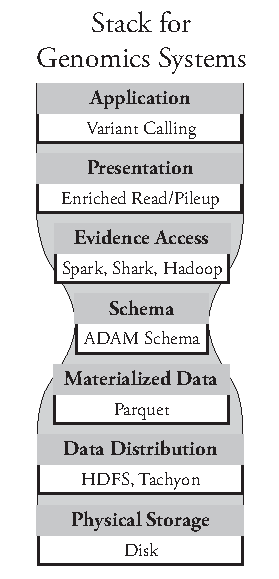
\includegraphics[width=0.4\linewidth]{stack-model.pdf}
\end{center}
\caption{A Stack Model for Genomics}
\label{fig:stack-model}
\end{figure}

The seven layers of our stack model are decomposed as follows, traditionally numbered from bottom to top:

\begin{enumerate}
\item {\bf Physical Storage:} This layer coordinates data writes to physical media, usually magnetic disk.
\item {\bf Data Distribution:} This layer manages access, replication, and distribution of the genomics files that have been written to disk.
\item {\bf Materialized Data:} This layer encodes the patterns for how data is encoded and stored. This provides read/write efficiency
and compression.
\item {\bf Data Schema:} This layer specifies the representation of data when it is accessed, and forms the narrow waist of the pipeline.
\item {\bf Evidence Access:} This layer implements efficient methods for performing common access patterns such as random database
queries, or sequential/parallel reading of records from a flat file.
\item {\bf Presentation:} The presentation layer provides the application developer with efficient and
straightforward methods for querying the characteristics of individual portions of genetic data.
\item {\bf Application:} Applications like variant calling and alignment are implemented in this layer.
\end{enumerate}

The ADAM schema is represented using Apache Avro~\citep{avro}, which is an open-source, cross-platform data serialization framework, similar
to Apache Thrift and Google's Protocol Buffers~\citep{thrift, protobuf}. Avro was chosen as the interchange format for several reasons:

\begin{itemize}
\item Avro is an open-source framework covered by the Apache 2 license. This means that Avro can be used in both open and closed source software.
\item Avro has broad cross-platform support. Natively, Avro supports C/C++/C\#, Java, Scala, Python, Ruby, and php.
\item Avro provides a clear and human readable language for explicitly describing the schema of an object~(Avro Description Language, AVDL).
\item Avro is natively supported by several common map-reduce frameworks and database systems.
\item Avro schemas can be updated without breaking compatibility with objects written using a previous version of the schema.
\end{itemize}

As noted above, for a system to implement the ADAM format, it must read/write ADAM objects that are defined by Avro schemas. This minimizes
tool/vendor lock-in.

A well defined software stack has several significant advantages. By limiting application interactions with layers lower than the presentation layer,
application developers are given a clear and consistent view of the data they are processing. By divorcing the API from the data
access layer, we unlock significant flexibility. With careful design in the data format and data access layers, we can seamlessly
support conventional flat file access patterns, while also allowing easy access to data with database methods. By treating the
compute substrate and storage as separate layers, we also drastically increase the portability of the APIs that we implement.

\subsection{Reference Implementation}
\label{sec:reference-implementation}

In this paper, we present a reference implementation of a read processing pipeline~(\texttt{adam-core}). This implementation is fully open source
and is designed for a distributed, in-memory map-reduce framework. We do not optimize for a specific computing platform---rather, we have designed
agnostically for a commodity cloud computing platform. We discuss this decision in~\S\ref{sec:dedicated-clusters-vs-cloud-computing}. Our reference
implementation provides several read processing stages that can be either run from a command line, or executed by another application through
an API, as well as an API for enriched datatypes. These APIs are similar to those provided by SAMtools~\citep{li09} and Picard~\citep{picard}.

When we introduced the ADAM processing pipeline in~\S\ref{sec:introduction}, we noted that we built our system using the Avro data serialization
format, the Parquet columnar store, and the Spark map-reduce framework~\citep{avro, parquet, zaharia10}. The rationale for using Avro was
introduced in the prior section---in this section, we will address why we chose to use Parquet and Spark.

\paragraph{Spark, In-Memory Map-Reduce:}
\label{sec:spark}

As introduced in \citet{zaharia10} and further described in \citet{zaharia12}, Spark is an in-memory, distributed map-reduce framework that is
compatible with the Hadoop ecosystem and is open source under the Apache 2 license. Spark differs from conventional map-reduce frameworks
like Hadoop~\citep{hadoop} and Google MapReduce~\citep{dean08}, as it avoids writing data to disk whenever possible and instead caches
data in memory. This provides a dramatic speedup for iterative computations---Spark sees a 30--100$\times$ speedup on iterative jobs by eliminating
disk I/O and by improving resource utilization by pipelining computation. This pattern is a good fit for genomics:

\begin{itemize}
\item With the increasing size of genomic datasets, dsk I/O is a bottleneck for modern genomics systems. By persisting data in memory between processing stages,
we are able to lessen the disk I/O penalty and improve latency.
\item Many genomic processing stages are iterative. For many applications, iteration implies that stages can be pipelined, which improves system performance on large
parallel systems\footnote{Performance is improved as pipelining reduces the number of executors that become idle at the start and end of stages by overlapping the
two stages.}. 
\end{itemize}

An additional benefit of Spark is that its programming interface supports Java, Scala, and Python. A programming interface for the R programming language will
be available in the first half of 2014.

\paragraph{Parquet, Columnar File Format:}
\label{sec:parquet}

Parquet is a columnar file format that is designed for distributed computing. Columnar stores differ from conventional file formats as they group data together
by field instead of by record\footnote{In other words, all values for a single field are stored sequentially on disk.}. This enables very high read performance, improved
compression~\citep[see][]{abadi06}, and the efficient serialization of a subset of fields. Parquet has several additional benefits:

\begin{itemize}
\item Parquet operates by splitting a single ``file'' into many smaller files that contain \emph{row groups}\footnote{In Parquet, a \emph{row group} contains a subset
of rows of data from the dataset. The row groups are then stored in columnar format.}. This enables both parallelism by column and by row which increases read parallelism.
\item Parquet provides \emph{predicate pushdown}, where user defined filters are applied while records are being read. This can lead to a $>$2$\times$ performance increase.
A detailed analysis of Parquet's predicate pushdown functions for genomics applications can be found in \citet{massie13}.
\end{itemize}

Figure~\ref{fig:file-format} shows how ADAM in Parquet compares to BAM. We remove the file header from BAM, and instead distribute these values across all of the records
stored. This dissemination eliminates global information and makes the file much simpler to distribute across machines. This distribution is effectively free in a columnar store,
as the store just notes that the information is replicated across many reads.

\begin{figure}[h]
\begin{center}
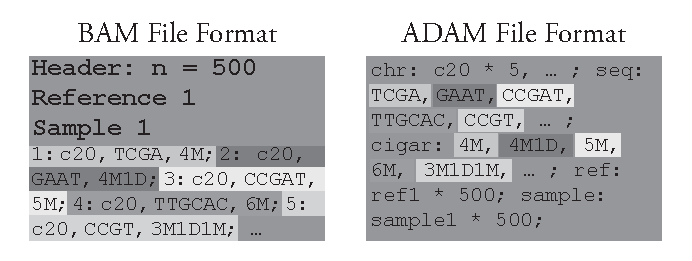
\includegraphics[width=\linewidth]{file-format.pdf}
\end{center}
\caption{Comparative Visualization of BAM and ADAM File Formats}
\label{fig:file-format}
\end{figure}

Our reference pipeline implementation provides two components:

\begin{itemize}
\item \texttt{adam-cli}, a command line toolkit for converting data to/from the ADAM format, and for performing transformations, and
\item \texttt{adam-core}, an API for processing genomic data that is stored in the ADAM format and is contained in memory.
\end{itemize}

We further describe the functionality provided by the command line toolkit and the API in~\S\ref{sec:data-transformations}.

\section{Methods}
\label{sec:methods}

ADAM contains formats for storing read and reference oriented sequence information, and variant/genotype data. The read oriented sequence format is forwards and
backwards compatible with BAM/SAM, and the variant/genotype data is forwards and backwards compatible with VCF. In this section, we discuss the specific data formats
that we provide. Additionally, we describe the \texttt{adam-cli} toolkit and \texttt{adam-core} API which were introduced in~\S\ref{sec:reference-implementation}.

\subsection{Data Format and Schema}
\label{sec:data-format-and-schema}

The data representation for the ADAM format is described using the open source Apache Avro data serialization system~\citep{avro}. The Avro system also provides a human
readable schema description language that can auto-generate the schema implementation in several common languages including C/C++/C\#, Java/Scala, php, Python, and
Ruby. This flexibility provides a significant cross-compatibility advantage over the BAM/SAM format, where the data format has only been implemented for C/C++ through
Samtools~\citep{li09} and for Java through Picard~\citep{picard}. Additionally, there are known incompatibilities between these different implementations---by using Avro,
we eliminate these platform compatibility issues.

The data types presented in this section make up the narrow waist of our proposed genomics stack in Figure \ref{fig:stack-model}. We provide the following primary datatypes:

\begin{itemize}
\item \textbf{ADAMRecord:} This datatype is for storing read data, and provides similar semantics to the read storage in SAM/BAM;
\item \textbf{ADAMPileup:} This datatype stores reference-oriented pileup data, broken out by individual read base;
\item \textbf{ADAMGenotype:} This datatype represents the genotype of a single chromosome of a single sample; and
\item \textbf{ADAMVariant:} This datatype represents a single variant allele which segregates at a site.
\end{itemize}

In this section, we discuss novel details of our format implementation, and contrast the structure of our formats against the current BAM and VCF formats. We do not provide
a full description of all fields in our standard---a full description of the fields of the data types is available in the ADAM technical report~\citep[see][\S5]{massie13}. We note that
the internal representations of the data may change at any point in time---for the most up to date schema, we refer readers to the ADAM repository.

\paragraph{ADAMRecord, DNA Sequence Data:}
\label{sec:adamrecord}

An individual ADAMRecord is equivalent to a single read stored in SAM/BAM format. To improve parallelism, we eliminate the need for header references. This is done by
replicating the information that is contained in the header across all records. While this would be too expensive to implement in a traditional row-oriented file format, the use
of a columnar storage format like Parquet allows us to use run-length encoding~(RLE) to make this tractable. RLE is an efficient method that encodes that a single piece of
information is replicated across many~(not necessarily all) records. Even though we replicate the header information across all records, ADAMRecord data consumes less
space than BAM---ADAMRecord files are between 2\% and 25\% smaller than a compressed BAM file.

\paragraph{ADAMPileup, Locus-Oriented DNA Data:}
\label{sec:adampileup}

ADAM's pileup storage format stores individual read bases. This contrasts with traditional pileup formats which instead store all the bases which are found at a single reference
position. There are several reasons that inform this choice:

\begin{itemize}
\item By storing individual bases separately, it is easier to use database methods to query across reference oriented data.
\item We provide more intuitive formats for storing reference oriented insertion/deletion data. Specifically, our pileup storage format provides gap-based indexing, which
disambiguates the length of a deletion or insertion.
\item From the single read base format we provide, read data can be reconstructed losslessly from pileup data.
\end{itemize}

We do realize that many users are interested in viewing bases through the traditional pileup view. We provide an internal representation~(\textit{ADAMRod}) that provides
efficient access to this data.

Additionally, we provide \emph{pileup aggregation}, a technique that is similar to \texttt{ReducedReads}~\citep[see][]{mckenna10}. Pileup aggregation takes all bases that
share a base type~(e.g. cytosine, guanine, etc.), and averages their statistical values. This technique is useful in some circumstances~(e.g. data archival) as it leads to a
reduction in the amount of data stored that scales approximately as $O(1/coverage)$.

\paragraph{ADAMGenotype, Single Chromosome Genotypes, and ADAMVariant, Multi-Sample Variant Data:}
\label{sec:adamvariant}

ADAM implements genotypes without relying on the context of a variant. An individual ADAMGenotype record describes a called genotype on a single chromosome of a
sample. The metrics fields of a genotype~(e.g. quality) mirror the metrics fields of the variant type. This enables genotypes to be expressed without the centralized notion
of a variant---this is useful for data warehousing, where the genotypes of many samples may be gathered. At a later point in time, it may be desirable to collect and distribute
variant calls for a subset of these samples; this subset may span multiple variant calling runs. By mirroring fields between Genotype and Variant records, we allow ourselves
to compute variant statistics from a set of genotypes without having access to the raw read data. This transformation is implemented in both the \texttt{adam-cli} and the
\texttt{adam-core} API.

Annotations are not a first class citizen of the VCF format---annotations are shoehorned in to the format through the use of the attributes field. For ADAMGenotypes and
ADAMVariants, we allow users to define record schemas that are not part of the core variant/genotype schemas. We then additionally provide an internal ADAMVariantContext
class that unifies annotations with specific genotypes and variants. Annotations are typically unified through the use of user defined \emph{joins}, which are a database
construct. There are several advantages to this process:

\begin{itemize}
\item Since users are defining records for annotations, annotated data can now be more complex---specifically, annotated data can contain multiple fields, or complex fields.
\item As the \emph{joins} are user defined, no limitations are placed on the forms of annotations that are provided. Annotations can be specific to a site, variant, genotype,
sample, or etc.
\end{itemize}

Additionally, since annotations are defined through an explicit schema, annotation maintenance becomes significantly simpler.

\paragraph{ADAM Sequence Dictionaries:}
\label{sec:adam-sequence-dictionaries}

\textbf{Timothy, can you write this?}

\subsection{Data Transformations}
\label{sec:data-transformations}

In this section, we provide a brief discussion of the transforms and utilities implemented inside of ADAM. For an extended description of the \textit{Sorting}, \textit{Mark
Duplicates}, \textit{BQSR}, and \textit{Indel Realignment} algorithms, we refer readers to the appendix of \citet{massie13} which discusses these algorithms in more detail.
We discuss the command line utilities that we provide, and give a brief overview of some of the transformations that our API provides.

\paragraph{Command Line Utilities:}
\label{sec:command-line-utilities}

The \texttt{adam-cli} suite of command line utilities implements several important features. They include:

\begin{itemize}
\item Converters between:
\begin{itemize}
\item ADAMRecord $\leftrightarrow$ SAM/BAM
\item ADAMVariant and ADAMGenotype $\leftrightarrow$ VCF
\item ADAMRecord $\rightarrow$ ADAMPileup
\item ADAMRecord $\rightarrow$ SAMtools style pileups 
\end{itemize}
\item \textit{AggregatePileups}, which aggregates pileup data~(see~\S\ref{sec:adampileup}),
\item \textit{CompareAdam}, which compares two ADAM read files,
\item \textit{ComputeVariants}, which computes variant data from a set of genotypes~(see~\S\ref{sec:adamvariant}),
\item \textit{Flagstat}, which is analogous to SAMtools' \texttt{flagstat} command,
\item \textit{ListDict}, which lists the content of an ADAM sequence dictionary,
\item \textit{PrintAdam}, which prints the contents of an ADAMRecord file, and
\item \textit{Transform}, which allows users to perform sorting, duplicate marking, and BQSR on read data.
\end{itemize}

The translations between ADAM and SAM/BAM/VCF use the Hadoop-BAM framework~\citep[see][]{niemenmaa12} to read and write SAM/BAM/VCF data---this allows for these
translations to be distributed, which accelerates the translations. Similarly, all of the commands that operate on read data can operate on ADAMRecord, SAM, or BAM data;
if SAM or BAM data is provided, it is transformed on-demand into ADAMRecords.

\paragraph{API Transformations:}
\label{sec:api-transforms}

The \texttt{adam-core} API provides an extensive set of transformations that are performed on data stored in Resilient Distributed Dataset~(RDD) form. RDDs were introduced
in \citet{zaharia12} as a fault-tolerant abstraction for distributing an array of data across multiple machines. The API transformations we provide form the base on which the
\texttt{adam-cli} is built. Some important transformations provided by our API include:

\begin{itemize}
\item Read data:
\begin{itemize}
\item Sort by reference position
\item Mark Duplicates
\item BQSR
\item Realign Indels
\item Collect reference sequence dictionary
\item Collect metrics
\item Translate reads to pileups
\end{itemize}
\item Pileup data:
\begin{itemize}
\item Aggregate pileup data
\item Group pileups by reference position
\item Seperate reference position grouped data by samples
\item Compute coverage metrics
\end{itemize}
\item Genotype data:
\begin{itemize}
\item Validate multi-sample genotype data
\item Compute variant data from genotypes
\end{itemize}
\end{itemize}

Additionally, our API provides several enriched datatypes that provide better access semantics for developers. These enriched types include:

\begin{itemize}
\item \textit{ADAMVariantContext}, a type which unifies variant, genotype, and annotation data;
\item \textit{RichADAMRecord}, a wrapper around ADAMRecords that converts some fields into richer record types (e.g. CIGAR/MD strings);
\item \textit{ADAMRod}, a type that wraps pileup bases at a single locus position;
\item \textit{MdTag}s, an enriched class for accessing alignment mismatch data; and,
\item \textit{ReferencePosition}, \textit{ReferencePositionPair}, and \textit{ReferenceRegion}, which are helper classes that provide rich semantics for describing the relationship
between an object and it's location on the reference genome.
\end{itemize}

The \texttt{adam-core} API also provides partitioners for reference-aligned data. These partitioners work with the Spark map-reduce framework to efficiently co-locate data that
has spatial locality. This improves the performance of applications that operate on data with high spatial locality by improving the likelihood that two objects that have high
locality on the reference genome will be on the same machine. This reduces the amount of data that must be fetched across the network when performing distributed computing.

\subsection{Performance}
\label{sec:performance}

Table~\ref{tab:overview} previews the performance of ADAM for \textit{Sort} and \textit{Mark Duplicates}.

\begin{table}[h]
\processtable{\textit{Sort} and \textit{Mark Duplicates} Performance on NA12878\label{tab:overview}}
{\begin{tabular}{ l c c }
\toprule
\bf Software & \bf EC2 profile & \bf Wall Clock Time \\
\midrule
Picard 1.103 & 1 \texttt{hs1.8xlarge} & 17h 44m \\
ADAM 0.5.0 & 1 \texttt{hs1.8xlarge} & 8h 56m \\
ADAM 0.5.0 & 32 \texttt{cr1.8xlarge} & 33m \\
ADAM 0.5.0 & 100 \texttt{m2.4xlarge} & 21m \\ 
\midrule
\bf Software & \bf EC2 profile & \bf Wall Clock Time \\
\midrule
Picard 1.103 & 1 \texttt{hs1.8xlarge} & 20h 22m \\
ADAM 0.5.0 & 100 \texttt{m2.4xlarge} & 29m \\
\botrule
\end{tabular}}{}
\end{table}

\section{Discussion}
\label{sec:discussion}

\begin{table}[h]
\processtable{Comparison of File Formats\label{tab:comparison}}
{\begin{tabular}{ l c c }
\toprule
 & \bf BAM & \bf ADAM \\
\midrule
\bf Size & 1.0$\times$ & 0.75-0.9$\times$ \\
\bf Scalability & $<$8 machines & $>$100 machines \\
\midrule
& \bf VCF & \bf ADAM \\
\midrule
\bf Scalability & $<$8 machines & $>$100 machines \\
\botrule
\end{tabular}}{}
\end{table}

\subsection{Single Node Processing vs. Dedicated Clusters vs. Cloud Computing}
\label{sec:single-vs-clusters-vs-cloud}

A central goal during the development of ADAM was to not force users to follow specific patterns. As such, we have also made efforts to design the ADAM format and command
line utilities to be portable across different computing installations. We envision that end users will be using ADAM either on a single workstation, on a dedicated computing
cluster, or through a cloud computing provider like Amazon EC2 or Microsoft Azure. As can be seen in~\S\ref{sec:performance}, ADAM performs admirably on all platforms,
achieving a 2$\times$ speedup over the current state-of-the-art on a single node, and near-linear speedup on when distributed.

As traditional genomics workflows could not easily or efficiently use compute clusters, many users have performed the bulk of their processing on beefy workstations. We predict
that the rise of distributed computing tools for genomics will soon render workstations uneconomical. Instead, we expect that clinical/research centers who process consistently
high volumes of genomic data will build and maintain their own dedicated compute farms. For clinical and research groups that do process genomic data, but not a sufficient
amount to justify the cost of a cluster, cloud computing platforms are attractive:

\begin{itemize}
\item Commercial cloud platforms are economically attractive as they do not present any capital acquisition costs, nor do they have maintenance costs. Additionally, cloud
platforms tend to offer several levels of service differentiation:
\begin{itemize}
\item Users can trade cost for performance, as the number of machines and performance of machines can be selected,
\item Cloud platforms also frequently auction unused slots off at below-market prices\footnote{For Amazon EC2, these are known as \emph{spot instances}.}, which can
further reduce costs.
\end{itemize}
\item System setup can be simplified through the use of systems like \textit{Docker}~\citep{docker} for distributing consistent application images.
\item Inexpensive pay-as-you-go storage solutions are available which provide good performance when used with a cloud service.
\end{itemize}

We anticipate that formats like ADAM will ease this transition, as ADAM can be used efficiently on all platforms. Additionally, ADAM's stack model explicitly allows for significant
flexibility in the format. This will allow ADAM to easily adapt to any future computing revolutions.

\subsection{Evolution of Standard}
\label{sec:evolution-of-standard}

ADAM's read, pileup, variant, and genotype formats are designed to evolve cleanly. The formats are easy to evolve because they are expressed as an explicit schema
in Avro. Avro allows for an application that has been compiled against a specific version of the schema to read data that has been written in an older or newer version of the
schema, as long as a simple process is followed when updating the schema.

Additionally, we have designed the formats to allow for user defined fields to be added without changing the core schema. Read data uses ``attributes,'' in a fashion similar to
the SAM/BAM format. For variant and genotype data, our variant context implementation~(see~\S\ref{sec:adamvariant}) supports several different and expressive ways for
defining new fields. The variant context method is superior to the annotations provided by the VCF standard, as it provides higher expressivity while promoting better
organization.

ADAM is a community effort, and all members of the community are invited to modify both the data formats and the processing pipelines. The ADAM team has established a
Request For Comment~(RFC) system that is similar to the one used by the Internet Engineering Task Force~(IETF). Here, modifications are proposed and opened for public
discussion for a set time frame. After a consensus is reached, the format can be amended. The RFC platform is hosted at our project
website\footnote{\url{http://adam.cs.berkeley.edu/rfc}}.

\section{Conclusion}
\label{sec:conclusion}

This paper presents ADAM, a new data storage format and processing pipeline for genomics data. Our reference implementation makes use of efficient columnar storage
systems to improve the lossless compression available for storing read data, and uses in-memory processing techniques to eliminate the read processing bottleneck faced by
modern genomics pipelines. We also present APIs that enhance developer access to read, pileup, genotype, and variant data.

We are currently in the process of extending ADAM to support SQL querying of genomic data, and extending our transformations API to more programming languages. 
ADAM promises to improve the development of applications that process genomic data, by removing current difficulties with the extraction and loading of data and by
providing simple and performant programming abstractions for processing this data at scale.

\section*{Acknowledgement}
\label{sec:acknowledgement}

The authors would like to thank their many colleagues who provided feedback on early implementations of ADAM, and on drafts of the manuscript. Additionally, we would
like to thank Uri Laserson, David Haussler, Adam Novak, Mauricio Carnerio, and Joel Thibault for their feedback on technical direction and format implementation.

\paragraph{Funding\textcolon}
\label{sec:funding}

This research is supported in part by NSF CISE Expeditions award CCF-1139158 and DARPA XData Award FA8750-12-2-0331, a NSF
Graduate Research Fellowship (DGE-1106400) and gifts from Amazon Web Services, Google, SAP,  Apple, Inc., Cisco, Clearstory Data,
Cloudera, Ericsson, Facebook, GameOnTalis, General Electric, Hortonworks, Huawei, Intel, Microsoft, NetApp, Oracle, Samsung, Splunk,
VMware, WANdisco and Yahoo!.

\bibliographystyle{natbib}

\bibliography{adam-ismb-2013}

\end{document}
